\documentclass[1p]{elsarticle_modified}
%\bibliographystyle{elsarticle-num}

%\usepackage[colorlinks]{hyperref}
%\usepackage{abbrmath_seonhwa} %\Abb, \Ascr, \Acal ,\Abf, \Afrak
\usepackage{amsfonts}
\usepackage{amssymb}
\usepackage{amsmath}
\usepackage{amsthm}
\usepackage{scalefnt}
\usepackage{amsbsy}
\usepackage{kotex}
\usepackage{caption}
\usepackage{subfig}
\usepackage{color}
\usepackage{graphicx}
\usepackage{xcolor} %% white, black, red, green, blue, cyan, magenta, yellow
\usepackage{float}
\usepackage{setspace}
\usepackage{hyperref}

\usepackage{tikz}
\usetikzlibrary{arrows}

\usepackage{multirow}
\usepackage{array} % fixed length table
\usepackage{hhline}

%%%%%%%%%%%%%%%%%%%%%
\makeatletter
\renewcommand*\env@matrix[1][\arraystretch]{%
	\edef\arraystretch{#1}%
	\hskip -\arraycolsep
	\let\@ifnextchar\new@ifnextchar
	\array{*\c@MaxMatrixCols c}}
\makeatother %https://tex.stackexchange.com/questions/14071/how-can-i-increase-the-line-spacing-in-a-matrix
%%%%%%%%%%%%%%%

\usepackage[normalem]{ulem}

\newcommand{\msout}[1]{\ifmmode\text{\sout{\ensuremath{#1}}}\else\sout{#1}\fi}
%SOURCE: \msout is \stkout macro in https://tex.stackexchange.com/questions/20609/strikeout-in-math-mode

\newcommand{\cancel}[1]{
	\ifmmode
	{\color{red}\msout{#1}}
	\else
	{\color{red}\sout{#1}}
	\fi
}

\newcommand{\add}[1]{
	{\color{blue}\uwave{#1}}
}

\newcommand{\replace}[2]{
	\ifmmode
	{\color{red}\msout{#1}}{\color{blue}\uwave{#2}}
	\else
	{\color{red}\sout{#1}}{\color{blue}\uwave{#2}}
	\fi
}

\newcommand{\Sol}{\mathcal{S}} %segment
\newcommand{\D}{D} %diagram
\newcommand{\A}{\mathcal{A}} %arc


%%%%%%%%%%%%%%%%%%%%%%%%%%%%%5 test

\def\sl{\operatorname{\textup{SL}}(2,\Cbb)}
\def\psl{\operatorname{\textup{PSL}}(2,\Cbb)}
\def\quan{\mkern 1mu \triangleright \mkern 1mu}

\theoremstyle{definition}
\newtheorem{thm}{Theorem}[section]
\newtheorem{prop}[thm]{Proposition}
\newtheorem{lem}[thm]{Lemma}
\newtheorem{ques}[thm]{Question}
\newtheorem{cor}[thm]{Corollary}
\newtheorem{defn}[thm]{Definition}
\newtheorem{exam}[thm]{Example}
\newtheorem{rmk}[thm]{Remark}
\newtheorem{alg}[thm]{Algorithm}

\newcommand{\I}{\sqrt{-1}}
\begin{document}

%\begin{frontmatter}
%
%\title{Boundary parabolic representations of knots up to 8 crossings}
%
%%% Group authors per affiliation:
%\author{Yunhi Cho} 
%\address{Department of Mathematics, University of Seoul, Seoul, Korea}
%\ead{yhcho@uos.ac.kr}
%
%
%\author{Seonhwa Kim} %\fnref{s_kim}}
%\address{Center for Geometry and Physics, Institute for Basic Science, Pohang, 37673, Korea}
%\ead{ryeona17@ibs.re.kr}
%
%\author{Hyuk Kim}
%\address{Department of Mathematical Sciences, Seoul National University, Seoul 08826, Korea}
%\ead{hyukkim@snu.ac.kr}
%
%\author{Seokbeom Yoon}
%\address{Department of Mathematical Sciences, Seoul National University, Seoul, 08826,  Korea}
%\ead{sbyoon15@snu.ac.kr}
%
%\begin{abstract}
%We find all boundary parabolic representation of knots up to 8 crossings.
%
%\end{abstract}
%\begin{keyword}
%    \MSC[2010] 57M25 
%\end{keyword}
%
%\end{frontmatter}

%\linenumbers
%\tableofcontents
%
\newcommand\colored[1]{\textcolor{white}{\rule[-0.35ex]{0.8em}{1.4ex}}\kern-0.8em\color{red} #1}%
%\newcommand\colored[1]{\textcolor{white}{ #1}\kern-2.17ex	\textcolor{white}{ #1}\kern-1.81ex	\textcolor{white}{ #1}\kern-2.15ex\color{red}#1	}

{\Large $\underline{12a_{0719}~(K12a_{0719})}$}

\setlength{\tabcolsep}{10pt}
\renewcommand{\arraystretch}{1.6}
\vspace{1cm}\begin{tabular}{m{100pt}>{\centering\arraybackslash}m{274pt}}
\multirow{5}{120pt}{
	\centering
	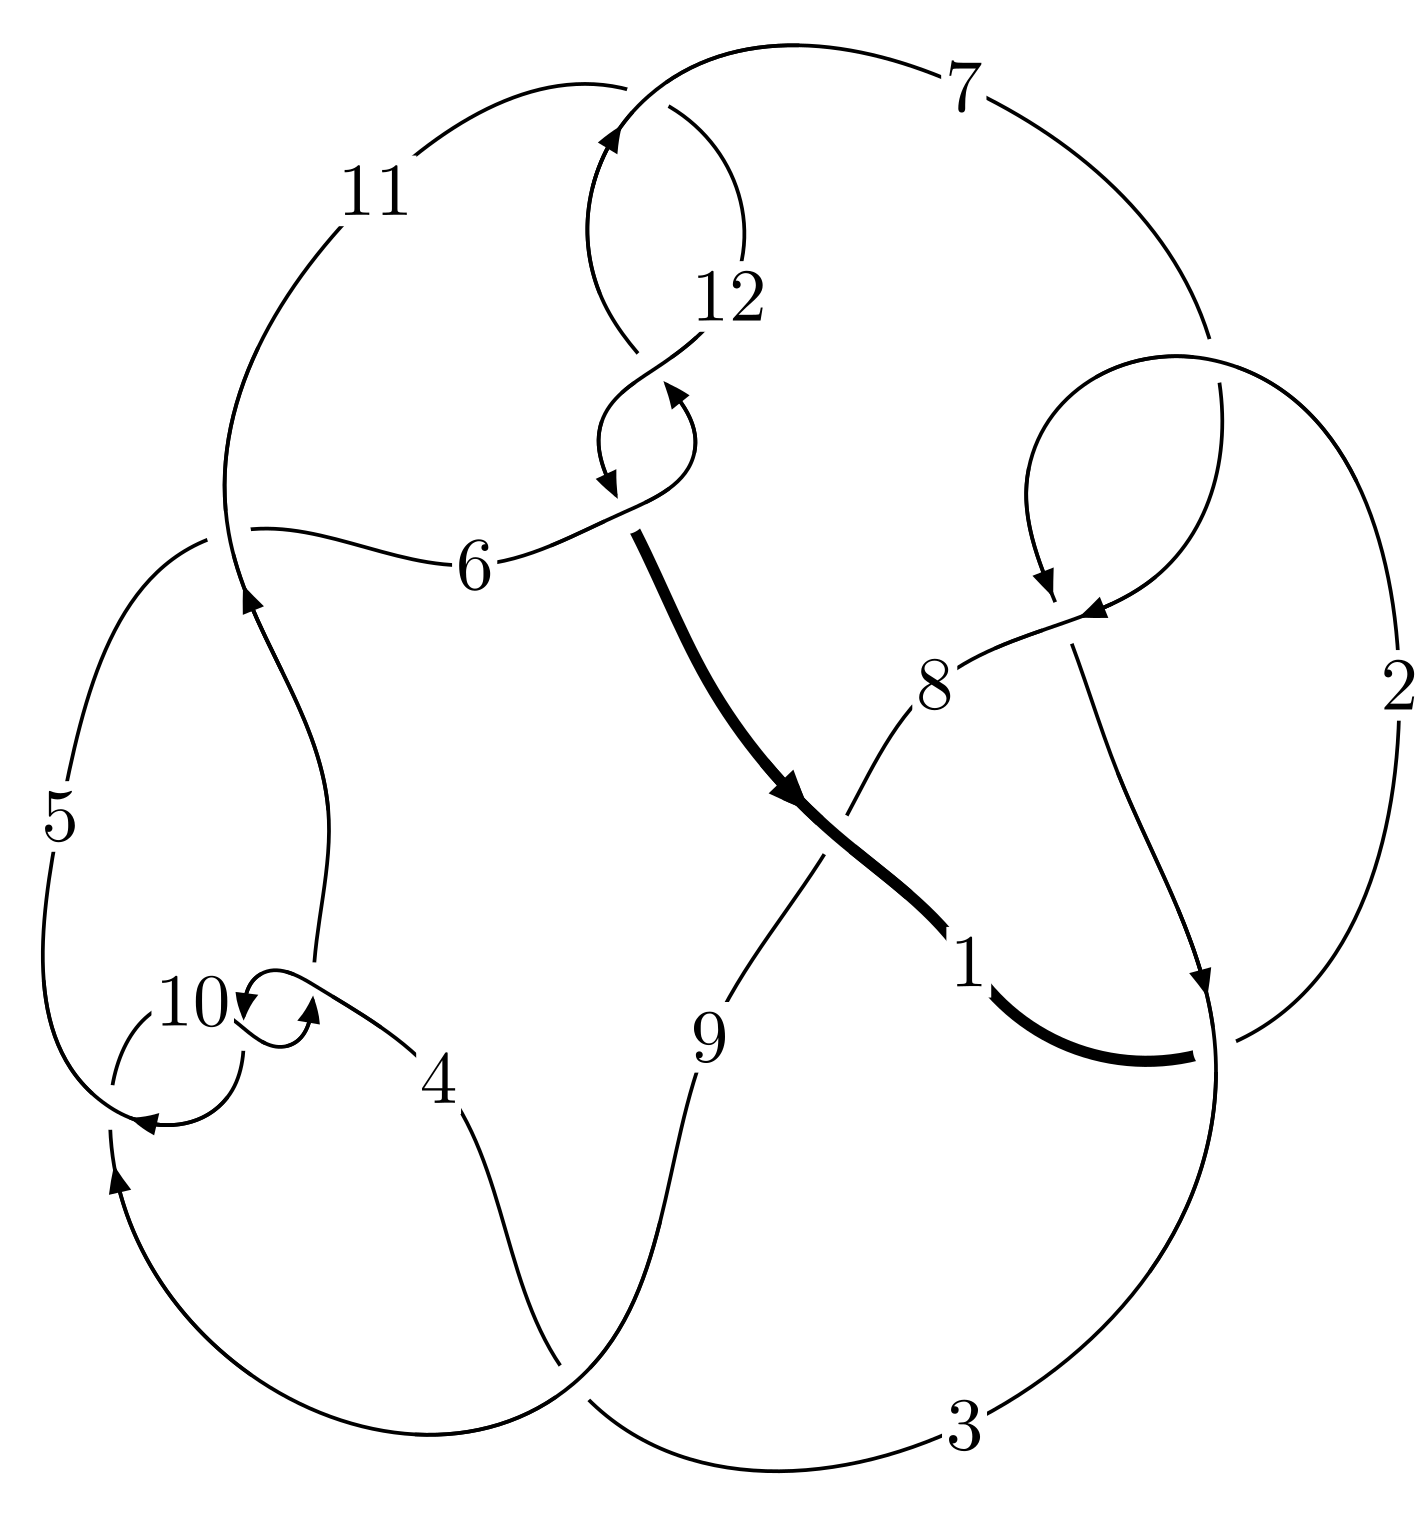
\includegraphics[width=112pt]{../../../GIT/diagram.site/Diagrams/png/1520_12a_0719.png}\\
\ \ \ A knot diagram\footnotemark}&
\allowdisplaybreaks
\textbf{Linearized knot diagam} \\
\cline{2-2}
 &
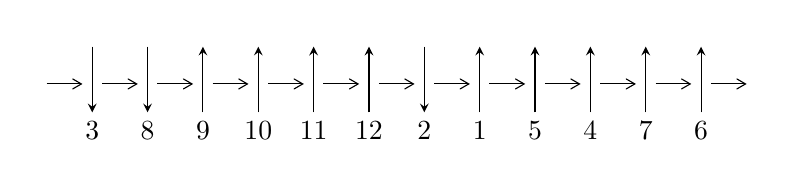
\begin{tikzpicture}[x=20pt, y=17pt]
	% nodes
	\node (C0) at (0, 0) {};
	\node (C1) at (1, 0) {};
	\node (C1U) at (1, +1) {};
	\node (C1D) at (1, -1) {3};

	\node (C2) at (2, 0) {};
	\node (C2U) at (2, +1) {};
	\node (C2D) at (2, -1) {8};

	\node (C3) at (3, 0) {};
	\node (C3U) at (3, +1) {};
	\node (C3D) at (3, -1) {9};

	\node (C4) at (4, 0) {};
	\node (C4U) at (4, +1) {};
	\node (C4D) at (4, -1) {10};

	\node (C5) at (5, 0) {};
	\node (C5U) at (5, +1) {};
	\node (C5D) at (5, -1) {11};

	\node (C6) at (6, 0) {};
	\node (C6U) at (6, +1) {};
	\node (C6D) at (6, -1) {12};

	\node (C7) at (7, 0) {};
	\node (C7U) at (7, +1) {};
	\node (C7D) at (7, -1) {2};

	\node (C8) at (8, 0) {};
	\node (C8U) at (8, +1) {};
	\node (C8D) at (8, -1) {1};

	\node (C9) at (9, 0) {};
	\node (C9U) at (9, +1) {};
	\node (C9D) at (9, -1) {5};

	\node (C10) at (10, 0) {};
	\node (C10U) at (10, +1) {};
	\node (C10D) at (10, -1) {4};

	\node (C11) at (11, 0) {};
	\node (C11U) at (11, +1) {};
	\node (C11D) at (11, -1) {7};

	\node (C12) at (12, 0) {};
	\node (C12U) at (12, +1) {};
	\node (C12D) at (12, -1) {6};
	\node (C13) at (13, 0) {};

	% arrows
	\draw[->,>={angle 60}]
	(C0) edge (C1) (C1) edge (C2) (C2) edge (C3) (C3) edge (C4) (C4) edge (C5) (C5) edge (C6) (C6) edge (C7) (C7) edge (C8) (C8) edge (C9) (C9) edge (C10) (C10) edge (C11) (C11) edge (C12) (C12) edge (C13) ;	\draw[->,>=stealth]
	(C1U) edge (C1D) (C2U) edge (C2D) (C3D) edge (C3U) (C4D) edge (C4U) (C5D) edge (C5U) (C6D) edge (C6U) (C7U) edge (C7D) (C8D) edge (C8U) (C9D) edge (C9U) (C10D) edge (C10U) (C11D) edge (C11U) (C12D) edge (C12U) ;
	\end{tikzpicture} \\
\hhline{~~} \\& 
\textbf{Solving Sequence} \\ \cline{2-2} 
 &
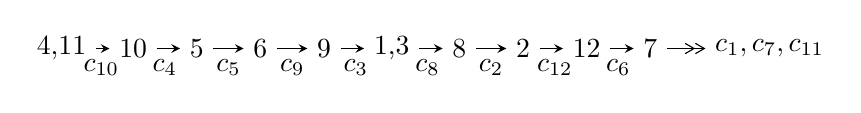
\begin{tikzpicture}[x=23pt, y=7pt]
	% node
	\node (A0) at (-1/8, 0) {4,11};
	\node (A1) at (1, 0) {10};
	\node (A2) at (2, 0) {5};
	\node (A3) at (3, 0) {6};
	\node (A4) at (4, 0) {9};
	\node (A5) at (81/16, 0) {1,3};
	\node (A6) at (49/8, 0) {8};
	\node (A7) at (57/8, 0) {2};
	\node (A8) at (65/8, 0) {12};
	\node (A9) at (73/8, 0) {7};
	\node (C1) at (1/2, -1) {$c_{10}$};
	\node (C2) at (3/2, -1) {$c_{4}$};
	\node (C3) at (5/2, -1) {$c_{5}$};
	\node (C4) at (7/2, -1) {$c_{9}$};
	\node (C5) at (9/2, -1) {$c_{3}$};
	\node (C6) at (45/8, -1) {$c_{8}$};
	\node (C7) at (53/8, -1) {$c_{2}$};
	\node (C8) at (61/8, -1) {$c_{12}$};
	\node (C9) at (69/8, -1) {$c_{6}$};
	\node (A10) at (11, 0) {$c_{1},c_{7},c_{11}$};

	% edge
	\draw[->,>=stealth]	
	(A0) edge (A1) (A1) edge (A2) (A2) edge (A3) (A3) edge (A4) (A4) edge (A5) (A5) edge (A6) (A6) edge (A7) (A7) edge (A8) (A8) edge (A9) ;
	\draw[->>,>={angle 60}]	
	(A9) edge (A10);
\end{tikzpicture} \\ 

\end{tabular} \\

\footnotetext{
The image of knot diagram is generated by the software ``\textbf{Draw programme}" developed by Andrew Bartholomew(\url{http://www.layer8.co.uk/maths/draw/index.htm\#Running-draw}), where we modified some parts for our purpose(\url{https://github.com/CATsTAILs/LinksPainter}).
}\phantom \\ \newline 
\centering \textbf{Ideals for irreducible components\footnotemark of $X_{\text{par}}$} 
 
\begin{align*}
I^u_{1}&=\langle 
u^4+2 u^2+b,\;u^{28}- u^{27}+\cdots+4 a-5,\;u^{29}+14 u^{27}+\cdots+u+1\rangle \\
I^u_{2}&=\langle 
-217988152638 u^{47}+1406532927108 u^{46}+\cdots+3784892885959 b-5225681996414,\\
\phantom{I^u_{2}}&\phantom{= \langle  }17960627004036 u^{47}-14379379524196 u^{46}+\cdots+3784892885959 a-93018602061573,\\
\phantom{I^u_{2}}&\phantom{= \langle  }u^{48}- u^{47}+\cdots-12 u+1\rangle \\
I^u_{3}&=\langle 
b-1,\;a^2+a u-1,\;u^2+1\rangle \\
\\
\end{align*}
\raggedright * 3 irreducible components of $\dim_{\mathbb{C}}=0$, with total 81 representations.\\
\footnotetext{All coefficients of polynomials are rational numbers. But the coefficients are sometimes approximated in decimal forms when there is not enough margin.}
\newpage
\renewcommand{\arraystretch}{1}
\centering \section*{I. $I^u_{1}= \langle u^4+2 u^2+b,\;u^{28}- u^{27}+\cdots+4 a-5,\;u^{29}+14 u^{27}+\cdots+u+1 \rangle$}
\flushleft \textbf{(i) Arc colorings}\\
\begin{tabular}{m{7pt} m{180pt} m{7pt} m{180pt} }
\flushright $a_{4}=$&$\begin{pmatrix}0\\u\end{pmatrix}$ \\
\flushright $a_{11}=$&$\begin{pmatrix}1\\0\end{pmatrix}$ \\
\flushright $a_{10}=$&$\begin{pmatrix}1\\u^2\end{pmatrix}$ \\
\flushright $a_{5}=$&$\begin{pmatrix}u\\u^3+u\end{pmatrix}$ \\
\flushright $a_{6}=$&$\begin{pmatrix}u^3+2 u\\u^3+u\end{pmatrix}$ \\
\flushright $a_{9}=$&$\begin{pmatrix}u^2+1\\u^4+2 u^2\end{pmatrix}$ \\
\flushright $a_{1}=$&$\begin{pmatrix}-\frac{1}{4} u^{28}+\frac{1}{4} u^{27}+\cdots-\frac{11}{2} u^2+\frac{5}{4}\\- u^4-2 u^2\end{pmatrix}$ \\
\flushright $a_{3}=$&$\begin{pmatrix}- u^5-2 u^3- u\\- u^7-3 u^5-2 u^3+u\end{pmatrix}$ \\
\flushright $a_{8}=$&$\begin{pmatrix}- u^{27}-\frac{1}{2} u^{26}+\cdots- u+\frac{1}{2}\\-\frac{1}{4} u^{28}+\frac{1}{4} u^{27}+\cdots+\frac{3}{2} u^2+\frac{1}{4}\end{pmatrix}$ \\
\flushright $a_{2}=$&$\begin{pmatrix}-\frac{1}{4} u^{28}+\frac{1}{4} u^{27}+\cdots-\frac{13}{2} u^2+\frac{5}{4}\\\frac{1}{4} u^{28}-\frac{1}{4} u^{27}+\cdots-\frac{1}{2} u^2-\frac{1}{4}\end{pmatrix}$ \\
\flushright $a_{12}=$&$\begin{pmatrix}-\frac{1}{4} u^{28}+\frac{1}{4} u^{27}+\cdots-\frac{7}{2} u^2+\frac{5}{4}\\- u^2\end{pmatrix}$ \\
\flushright $a_{7}=$&$\begin{pmatrix}\frac{1}{4} u^{28}+\frac{1}{4} u^{27}+\cdots+\frac{7}{2} u+\frac{1}{4}\\u\end{pmatrix}$\\&\end{tabular}
\flushleft \textbf{(ii) Obstruction class $= -1$}\\~\\
\flushleft \textbf{(iii) Cusp Shapes $= 2 u^{28}- u^{27}+27 u^{26}-10 u^{25}+159 u^{24}-38 u^{23}+522 u^{22}-51 u^{21}+990 u^{20}+75 u^{19}+912 u^{18}+361 u^{17}-172 u^{16}+442 u^{15}-1278 u^{14}-914 u^{12}-460 u^{11}+325 u^{10}-287 u^9+589 u^8+114 u^7+18 u^6+133 u^5-128 u^4+3 u^3+18 u^2-13 u+8$}\\~\\
\newpage\renewcommand{\arraystretch}{1}
\flushleft \textbf{(iv) u-Polynomials at the component}\newline \\
\begin{tabular}{m{50pt}|m{274pt}}
Crossings & \hspace{64pt}u-Polynomials at each crossing \\
\hline $$\begin{aligned}c_{1}\end{aligned}$$&$\begin{aligned}
&u^{29}+13 u^{28}+\cdots+17 u+4
\end{aligned}$\\
\hline $$\begin{aligned}c_{2},c_{7}\end{aligned}$$&$\begin{aligned}
&u^{29}+3 u^{28}+\cdots- u-2
\end{aligned}$\\
\hline $$\begin{aligned}c_{3},c_{5}\end{aligned}$$&$\begin{aligned}
&u^{29}-3 u^{28}+\cdots+80 u-32
\end{aligned}$\\
\hline $$\begin{aligned}c_{4},c_{6},c_{9}\\c_{10},c_{11},c_{12}\end{aligned}$$&$\begin{aligned}
&u^{29}+14 u^{27}+\cdots+u-1
\end{aligned}$\\
\hline $$\begin{aligned}c_{8}\end{aligned}$$&$\begin{aligned}
&u^{29}+9 u^{28}+\cdots+95 u+6
\end{aligned}$\\
\hline
\end{tabular}\\~\\
\newpage\renewcommand{\arraystretch}{1}
\flushleft \textbf{(v) Riley Polynomials at the component}\newline \\
\begin{tabular}{m{50pt}|m{274pt}}
Crossings & \hspace{64pt}Riley Polynomials at each crossing \\
\hline $$\begin{aligned}c_{1}\end{aligned}$$&$\begin{aligned}
&y^{29}+7 y^{28}+\cdots-271 y-16
\end{aligned}$\\
\hline $$\begin{aligned}c_{2},c_{7}\end{aligned}$$&$\begin{aligned}
&y^{29}-13 y^{28}+\cdots+17 y-4
\end{aligned}$\\
\hline $$\begin{aligned}c_{3},c_{5}\end{aligned}$$&$\begin{aligned}
&y^{29}-19 y^{28}+\cdots-7424 y-1024
\end{aligned}$\\
\hline $$\begin{aligned}c_{4},c_{6},c_{9}\\c_{10},c_{11},c_{12}\end{aligned}$$&$\begin{aligned}
&y^{29}+28 y^{28}+\cdots+y-1
\end{aligned}$\\
\hline $$\begin{aligned}c_{8}\end{aligned}$$&$\begin{aligned}
&y^{29}- y^{28}+\cdots+5569 y-36
\end{aligned}$\\
\hline
\end{tabular}\\~\\
\newpage\flushleft \textbf{(vi) Complex Volumes and Cusp Shapes}
$$\begin{array}{c|c|c}  
\text{Solutions to }I^u_{1}& \I (\text{vol} + \sqrt{-1}CS) & \text{Cusp shape}\\
 \hline 
\begin{aligned}
u &= -0.837271 + 0.076877 I \\
a &= -2.37885 + 0.65426 I \\
b &= -1.85683 + 0.43644 I\end{aligned}
 & \phantom{-}4.96568 - 6.65204 I & \phantom{-}9.90546 + 5.57516 I \\ \hline\begin{aligned}
u &= -0.837271 - 0.076877 I \\
a &= -2.37885 - 0.65426 I \\
b &= -1.85683 - 0.43644 I\end{aligned}
 & \phantom{-}4.96568 + 6.65204 I & \phantom{-}9.90546 - 5.57516 I \\ \hline\begin{aligned}
u &= \phantom{-}0.833662 + 0.041563 I \\
a &= -2.37643 - 0.35224 I \\
b &= -1.86234 - 0.23468 I\end{aligned}
 & \phantom{-}6.73725 + 1.44483 I & \phantom{-}12.74743 - 0.59636 I \\ \hline\begin{aligned}
u &= \phantom{-}0.833662 - 0.041563 I \\
a &= -2.37643 + 0.35224 I \\
b &= -1.86234 + 0.23468 I\end{aligned}
 & \phantom{-}6.73725 - 1.44483 I & \phantom{-}12.74743 + 0.59636 I \\ \hline\begin{aligned}
u &= -0.732519\phantom{ +0.000000I} \\
a &= -1.59609\phantom{ +0.000000I} \\
b &= -1.36109\phantom{ +0.000000I}\end{aligned}
 & \phantom{-}1.48106\phantom{ +0.000000I} & \phantom{-}7.22880\phantom{ +0.000000I} \\ \hline\begin{aligned}
u &= \phantom{-}0.028083 + 1.284050 I \\
a &= -1.81534 - 0.31795 I \\
b &= \phantom{-}0.585292 + 0.093469 I\end{aligned}
 & -5.68843 + 2.62043 I & -0.80670 - 3.52599 I \\ \hline\begin{aligned}
u &= \phantom{-}0.028083 - 1.284050 I \\
a &= -1.81534 + 0.31795 I \\
b &= \phantom{-}0.585292 - 0.093469 I\end{aligned}
 & -5.68843 - 2.62043 I & -0.80670 + 3.52599 I \\ \hline\begin{aligned}
u &= \phantom{-}0.323515 + 1.266490 I \\
a &= \phantom{-}0.83700 - 1.78087 I \\
b &= \phantom{-}1.42217 + 0.81837 I\end{aligned}
 & -2.35148 + 1.67474 I & \phantom{-}2.52522 - 1.56718 I \\ \hline\begin{aligned}
u &= \phantom{-}0.323515 - 1.266490 I \\
a &= \phantom{-}0.83700 + 1.78087 I \\
b &= \phantom{-}1.42217 - 0.81837 I\end{aligned}
 & -2.35148 - 1.67474 I & \phantom{-}2.52522 + 1.56718 I \\ \hline\begin{aligned}
u &= -0.348532 + 1.291470 I \\
a &= \phantom{-}1.07285 + 1.53998 I \\
b &= \phantom{-}1.51186 - 0.98379 I\end{aligned}
 & -1.05837 - 7.04671 I & \phantom{-}4.61471 + 6.27988 I\\
 \hline 
 \end{array}$$\newpage$$\begin{array}{c|c|c}  
\text{Solutions to }I^u_{1}& \I (\text{vol} + \sqrt{-1}CS) & \text{Cusp shape}\\
 \hline 
\begin{aligned}
u &= -0.348532 - 1.291470 I \\
a &= \phantom{-}1.07285 - 1.53998 I \\
b &= \phantom{-}1.51186 + 0.98379 I\end{aligned}
 & -1.05837 + 7.04671 I & \phantom{-}4.61471 - 6.27988 I \\ \hline\begin{aligned}
u &= \phantom{-}0.133920 + 1.390120 I \\
a &= -0.659184 - 0.455120 I \\
b &= \phantom{-}0.302303 + 0.681001 I\end{aligned}
 & -9.06064 + 3.87312 I & -0.24533 - 3.24694 I \\ \hline\begin{aligned}
u &= \phantom{-}0.133920 - 1.390120 I \\
a &= -0.659184 + 0.455120 I \\
b &= \phantom{-}0.302303 - 0.681001 I\end{aligned}
 & -9.06064 - 3.87312 I & -0.24533 + 3.24694 I \\ \hline\begin{aligned}
u &= -0.380467 + 1.345060 I \\
a &= \phantom{-}1.37808 + 1.03819 I \\
b &= \phantom{-}1.60610 - 1.36006 I\end{aligned}
 & -2.01294 - 10.23390 I & \phantom{-}4.21079 + 5.73081 I \\ \hline\begin{aligned}
u &= -0.380467 - 1.345060 I \\
a &= \phantom{-}1.37808 - 1.03819 I \\
b &= \phantom{-}1.60610 + 1.36006 I\end{aligned}
 & -2.01294 + 10.23390 I & \phantom{-}4.21079 - 5.73081 I \\ \hline\begin{aligned}
u &= \phantom{-}0.338958 + 1.357740 I \\
a &= \phantom{-}0.987536 - 0.915157 I \\
b &= \phantom{-}1.31640 + 1.34118 I\end{aligned}
 & -7.32448 + 7.83990 I & -2.00524 - 4.89975 I \\ \hline\begin{aligned}
u &= \phantom{-}0.338958 - 1.357740 I \\
a &= \phantom{-}0.987536 + 0.915157 I \\
b &= \phantom{-}1.31640 - 1.34118 I\end{aligned}
 & -7.32448 - 7.83990 I & -2.00524 + 4.89975 I \\ \hline\begin{aligned}
u &= \phantom{-}0.39002 + 1.36214 I \\
a &= \phantom{-}1.47122 - 0.87684 I \\
b &= \phantom{-}1.63429 + 1.49453 I\end{aligned}
 & -4.1212 + 15.5713 I & \phantom{-}1.45377 - 9.68760 I \\ \hline\begin{aligned}
u &= \phantom{-}0.39002 - 1.36214 I \\
a &= \phantom{-}1.47122 + 0.87684 I \\
b &= \phantom{-}1.63429 - 1.49453 I\end{aligned}
 & -4.1212 - 15.5713 I & \phantom{-}1.45377 + 9.68760 I \\ \hline\begin{aligned}
u &= -0.08532 + 1.43102 I \\
a &= -0.804301 + 0.163541 I \\
b &= -0.023082 - 0.508186 I\end{aligned}
 & -13.00060 - 0.38893 I & -5.31626 - 0.21588 I\\
 \hline 
 \end{array}$$\newpage$$\begin{array}{c|c|c}  
\text{Solutions to }I^u_{1}& \I (\text{vol} + \sqrt{-1}CS) & \text{Cusp shape}\\
 \hline 
\begin{aligned}
u &= -0.08532 - 1.43102 I \\
a &= -0.804301 - 0.163541 I \\
b &= -0.023082 + 0.508186 I\end{aligned}
 & -13.00060 + 0.38893 I & -5.31626 + 0.21588 I \\ \hline\begin{aligned}
u &= -0.16556 + 1.42736 I \\
a &= -0.411189 + 0.278237 I \\
b &= \phantom{-}0.203418 - 0.954656 I\end{aligned}
 & -11.9273 - 8.4157 I & -3.46124 + 6.83368 I \\ \hline\begin{aligned}
u &= -0.16556 - 1.42736 I \\
a &= -0.411189 - 0.278237 I \\
b &= \phantom{-}0.203418 + 0.954656 I\end{aligned}
 & -11.9273 + 8.4157 I & -3.46124 - 6.83368 I \\ \hline\begin{aligned}
u &= \phantom{-}0.417850 + 0.314001 I \\
a &= \phantom{-}0.589467 - 1.254980 I \\
b &= -0.088921 - 0.564710 I\end{aligned}
 & -0.65256 + 3.97304 I & \phantom{-}7.14340 - 9.12328 I \\ \hline\begin{aligned}
u &= \phantom{-}0.417850 - 0.314001 I \\
a &= \phantom{-}0.589467 + 1.254980 I \\
b &= -0.088921 + 0.564710 I\end{aligned}
 & -0.65256 - 3.97304 I & \phantom{-}7.14340 + 9.12328 I \\ \hline\begin{aligned}
u &= -0.414438 + 0.109369 I \\
a &= \phantom{-}0.217260 + 0.434902 I \\
b &= -0.336911 + 0.210279 I\end{aligned}
 & \phantom{-}0.809813 - 0.139665 I & \phantom{-}12.95255 + 2.10646 I \\ \hline\begin{aligned}
u &= -0.414438 - 0.109369 I \\
a &= \phantom{-}0.217260 - 0.434902 I \\
b &= -0.336911 - 0.210279 I\end{aligned}
 & \phantom{-}0.809813 + 0.139665 I & \phantom{-}12.95255 - 2.10646 I \\ \hline\begin{aligned}
u &= \phantom{-}0.131847 + 0.393506 I \\
a &= \phantom{-}1.68992 - 0.55774 I \\
b &= \phantom{-}0.266797 - 0.179002 I\end{aligned}
 & -1.29100 - 1.59593 I & \phantom{-}3.66703 + 0.23498 I \\ \hline\begin{aligned}
u &= \phantom{-}0.131847 - 0.393506 I \\
a &= \phantom{-}1.68992 + 0.55774 I \\
b &= \phantom{-}0.266797 + 0.179002 I\end{aligned}
 & -1.29100 + 1.59593 I & \phantom{-}3.66703 - 0.23498 I\\
 \hline 
 \end{array}$$\newpage\newpage\renewcommand{\arraystretch}{1}
\centering \section*{II. $I^u_{2}= \langle -2.18\times10^{11} u^{47}+1.41\times10^{12} u^{46}+\cdots+3.78\times10^{12} b-5.23\times10^{12},\;1.80\times10^{13} u^{47}-1.44\times10^{13} u^{46}+\cdots+3.78\times10^{12} a-9.30\times10^{13},\;u^{48}- u^{47}+\cdots-12 u+1 \rangle$}
\flushleft \textbf{(i) Arc colorings}\\
\begin{tabular}{m{7pt} m{180pt} m{7pt} m{180pt} }
\flushright $a_{4}=$&$\begin{pmatrix}0\\u\end{pmatrix}$ \\
\flushright $a_{11}=$&$\begin{pmatrix}1\\0\end{pmatrix}$ \\
\flushright $a_{10}=$&$\begin{pmatrix}1\\u^2\end{pmatrix}$ \\
\flushright $a_{5}=$&$\begin{pmatrix}u\\u^3+u\end{pmatrix}$ \\
\flushright $a_{6}=$&$\begin{pmatrix}u^3+2 u\\u^3+u\end{pmatrix}$ \\
\flushright $a_{9}=$&$\begin{pmatrix}u^2+1\\u^4+2 u^2\end{pmatrix}$ \\
\flushright $a_{1}=$&$\begin{pmatrix}-4.74535 u^{47}+3.79915 u^{46}+\cdots-173.968 u+24.5763\\0.0575943 u^{47}-0.371618 u^{46}+\cdots-3.92085 u+1.38067\end{pmatrix}$ \\
\flushright $a_{3}=$&$\begin{pmatrix}- u^5-2 u^3- u\\- u^7-3 u^5-2 u^3+u\end{pmatrix}$ \\
\flushright $a_{8}=$&$\begin{pmatrix}-5.55732 u^{47}+3.55040 u^{46}+\cdots-170.824 u+25.8316\\-0.158538 u^{47}-0.442451 u^{46}+\cdots+4.87445 u-0.167244\end{pmatrix}$ \\
\flushright $a_{2}=$&$\begin{pmatrix}-3.20292 u^{47}+3.42884 u^{46}+\cdots-149.755 u+21.9747\\0.847526 u^{47}-0.612468 u^{46}+\cdots+3.21471 u+1.01524\end{pmatrix}$ \\
\flushright $a_{12}=$&$\begin{pmatrix}-3.50861 u^{47}+3.63777 u^{46}+\cdots-167.772 u+24.6986\\0.647166 u^{47}-0.266498 u^{46}+\cdots+1.13773 u+1.25150\end{pmatrix}$ \\
\flushright $a_{7}=$&$\begin{pmatrix}0.748497 u^{47}-0.101330 u^{46}+\cdots+20.5778 u-7.84423\\-0.251503 u^{47}+0.898670 u^{46}+\cdots-27.4222 u+4.15577\end{pmatrix}$\\&\end{tabular}
\flushleft \textbf{(ii) Obstruction class $= -1$}\\~\\
\flushleft \textbf{(iii) Cusp Shapes $= -\frac{24601630690532}{3784892885959} u^{47}+\frac{18604517425224}{3784892885959} u^{46}+\cdots-\frac{609246536515560}{3784892885959} u+\frac{112526788081386}{3784892885959}$}\\~\\
\newpage\renewcommand{\arraystretch}{1}
\flushleft \textbf{(iv) u-Polynomials at the component}\newline \\
\begin{tabular}{m{50pt}|m{274pt}}
Crossings & \hspace{64pt}u-Polynomials at each crossing \\
\hline $$\begin{aligned}c_{1}\end{aligned}$$&$\begin{aligned}
&(u^{24}+11 u^{23}+\cdots-2 u^2+1)^{2}
\end{aligned}$\\
\hline $$\begin{aligned}c_{2},c_{7}\end{aligned}$$&$\begin{aligned}
&(u^{24}- u^{23}+\cdots-2 u^3+1)^{2}
\end{aligned}$\\
\hline $$\begin{aligned}c_{3},c_{5}\end{aligned}$$&$\begin{aligned}
&(u^{24}+u^{23}+\cdots+10 u+1)^{2}
\end{aligned}$\\
\hline $$\begin{aligned}c_{4},c_{6},c_{9}\\c_{10},c_{11},c_{12}\end{aligned}$$&$\begin{aligned}
&u^{48}+u^{47}+\cdots+12 u+1
\end{aligned}$\\
\hline $$\begin{aligned}c_{8}\end{aligned}$$&$\begin{aligned}
&(u^{24}-3 u^{23}+\cdots-4 u+1)^{2}
\end{aligned}$\\
\hline
\end{tabular}\\~\\
\newpage\renewcommand{\arraystretch}{1}
\flushleft \textbf{(v) Riley Polynomials at the component}\newline \\
\begin{tabular}{m{50pt}|m{274pt}}
Crossings & \hspace{64pt}Riley Polynomials at each crossing \\
\hline $$\begin{aligned}c_{1}\end{aligned}$$&$\begin{aligned}
&(y^{24}+5 y^{23}+\cdots-4 y+1)^{2}
\end{aligned}$\\
\hline $$\begin{aligned}c_{2},c_{7}\end{aligned}$$&$\begin{aligned}
&(y^{24}-11 y^{23}+\cdots-2 y^2+1)^{2}
\end{aligned}$\\
\hline $$\begin{aligned}c_{3},c_{5}\end{aligned}$$&$\begin{aligned}
&(y^{24}-19 y^{23}+\cdots-48 y+1)^{2}
\end{aligned}$\\
\hline $$\begin{aligned}c_{4},c_{6},c_{9}\\c_{10},c_{11},c_{12}\end{aligned}$$&$\begin{aligned}
&y^{48}+35 y^{47}+\cdots-48 y+1
\end{aligned}$\\
\hline $$\begin{aligned}c_{8}\end{aligned}$$&$\begin{aligned}
&(y^{24}+y^{23}+\cdots+20 y+1)^{2}
\end{aligned}$\\
\hline
\end{tabular}\\~\\
\newpage\flushleft \textbf{(vi) Complex Volumes and Cusp Shapes}
$$\begin{array}{c|c|c}  
\text{Solutions to }I^u_{2}& \I (\text{vol} + \sqrt{-1}CS) & \text{Cusp shape}\\
 \hline 
\begin{aligned}
u &= -0.083162 + 1.035970 I \\
a &= \phantom{-}0.841864 - 0.321789 I \\
b &= -0.0601129 + 0.0367502 I\end{aligned}
 & -1.54603 - 2.05721 I & \phantom{-}8.27298 + 4.01793 I \\ \hline\begin{aligned}
u &= -0.083162 - 1.035970 I \\
a &= \phantom{-}0.841864 + 0.321789 I \\
b &= -0.0601129 - 0.0367502 I\end{aligned}
 & -1.54603 + 2.05721 I & \phantom{-}8.27298 - 4.01793 I \\ \hline\begin{aligned}
u &= \phantom{-}0.392939 + 0.971182 I \\
a &= -0.309360 - 0.748390 I \\
b &= \phantom{-}0.982133 - 0.443510 I\end{aligned}
 & -5.03285 + 0.40841 I & -1.87200 - 0.75563 I \\ \hline\begin{aligned}
u &= \phantom{-}0.392939 - 0.971182 I \\
a &= -0.309360 + 0.748390 I \\
b &= \phantom{-}0.982133 + 0.443510 I\end{aligned}
 & -5.03285 - 0.40841 I & -1.87200 + 0.75563 I \\ \hline\begin{aligned}
u &= \phantom{-}0.884347 + 0.132718 I \\
a &= \phantom{-}2.11818 + 1.02084 I \\
b &= \phantom{-}1.59566 + 1.20269 I\end{aligned}
 & \phantom{-}0.58237 + 11.00000 I & \phantom{-}5.31825 - 8.05284 I \\ \hline\begin{aligned}
u &= \phantom{-}0.884347 - 0.132718 I \\
a &= \phantom{-}2.11818 - 1.02084 I \\
b &= \phantom{-}1.59566 - 1.20269 I\end{aligned}
 & \phantom{-}0.58237 - 11.00000 I & \phantom{-}5.31825 + 8.05284 I \\ \hline\begin{aligned}
u &= -0.859254 + 0.109305 I \\
a &= \phantom{-}2.20088 - 0.78527 I \\
b &= \phantom{-}1.63876 - 1.06164 I\end{aligned}
 & \phantom{-}2.55519 - 5.78082 I & \phantom{-}8.37527 + 3.72629 I \\ \hline\begin{aligned}
u &= -0.859254 - 0.109305 I \\
a &= \phantom{-}2.20088 + 0.78527 I \\
b &= \phantom{-}1.63876 + 1.06164 I\end{aligned}
 & \phantom{-}2.55519 + 5.78082 I & \phantom{-}8.37527 - 3.72629 I \\ \hline\begin{aligned}
u &= -0.546029 + 0.650274 I \\
a &= -0.571077 + 0.256979 I \\
b &= \phantom{-}0.470130 - 0.014776 I\end{aligned}
 & -6.25412 + 1.34320 I & -2.02964 - 0.62000 I \\ \hline\begin{aligned}
u &= -0.546029 - 0.650274 I \\
a &= -0.571077 - 0.256979 I \\
b &= \phantom{-}0.470130 + 0.014776 I\end{aligned}
 & -6.25412 - 1.34320 I & -2.02964 + 0.62000 I\\
 \hline 
 \end{array}$$\newpage$$\begin{array}{c|c|c}  
\text{Solutions to }I^u_{2}& \I (\text{vol} + \sqrt{-1}CS) & \text{Cusp shape}\\
 \hline 
\begin{aligned}
u &= -0.649138 + 0.481545 I \\
a &= -0.151229 - 0.117560 I \\
b &= \phantom{-}0.508439 - 0.442655 I\end{aligned}
 & -5.72979 - 5.71321 I & -0.10823 + 7.50361 I \\ \hline\begin{aligned}
u &= -0.649138 - 0.481545 I \\
a &= -0.151229 + 0.117560 I \\
b &= \phantom{-}0.508439 + 0.442655 I\end{aligned}
 & -5.72979 + 5.71321 I & -0.10823 - 7.50361 I \\ \hline\begin{aligned}
u &= \phantom{-}0.784879 + 0.163524 I \\
a &= \phantom{-}1.66447 + 0.46022 I \\
b &= \phantom{-}1.33791 + 0.89026 I\end{aligned}
 & -2.54173 + 3.77265 I & \phantom{-}2.10807 - 3.49106 I \\ \hline\begin{aligned}
u &= \phantom{-}0.784879 - 0.163524 I \\
a &= \phantom{-}1.66447 - 0.46022 I \\
b &= \phantom{-}1.33791 - 0.89026 I\end{aligned}
 & -2.54173 - 3.77265 I & \phantom{-}2.10807 + 3.49106 I \\ \hline\begin{aligned}
u &= -0.795746 + 0.032611 I \\
a &= \phantom{-}2.46879 - 0.15993 I \\
b &= \phantom{-}1.74739 - 0.69246 I\end{aligned}
 & \phantom{-}3.07007 - 2.92383 I & \phantom{-}9.29020 + 3.29300 I \\ \hline\begin{aligned}
u &= -0.795746 - 0.032611 I \\
a &= \phantom{-}2.46879 + 0.15993 I \\
b &= \phantom{-}1.74739 + 0.69246 I\end{aligned}
 & \phantom{-}3.07007 + 2.92383 I & \phantom{-}9.29020 - 3.29300 I \\ \hline\begin{aligned}
u &= \phantom{-}0.469574 + 1.138130 I \\
a &= -0.062143 - 1.315650 I \\
b &= \phantom{-}1.41310 - 0.90321 I\end{aligned}
 & -2.49287 - 6.17959 I & \phantom{-0.000000 } 0 \\ \hline\begin{aligned}
u &= \phantom{-}0.469574 - 1.138130 I \\
a &= -0.062143 + 1.315650 I \\
b &= \phantom{-}1.41310 + 0.90321 I\end{aligned}
 & -2.49287 + 6.17959 I & \phantom{-0.000000 } 0 \\ \hline\begin{aligned}
u &= -0.423332 + 1.157340 I \\
a &= \phantom{-}0.118454 + 1.197480 I \\
b &= \phantom{-}1.54922 + 0.71748 I\end{aligned}
 & -0.655501 + 1.182900 I & \phantom{-0.000000 } 0 \\ \hline\begin{aligned}
u &= -0.423332 - 1.157340 I \\
a &= \phantom{-}0.118454 - 1.197480 I \\
b &= \phantom{-}1.54922 - 0.71748 I\end{aligned}
 & -0.655501 - 1.182900 I & \phantom{-0.000000 } 0\\
 \hline 
 \end{array}$$\newpage$$\begin{array}{c|c|c}  
\text{Solutions to }I^u_{2}& \I (\text{vol} + \sqrt{-1}CS) & \text{Cusp shape}\\
 \hline 
\begin{aligned}
u &= \phantom{-}0.763915 + 0.011868 I \\
a &= \phantom{-}2.60812 + 0.15719 I \\
b &= \phantom{-}1.78089 - 0.50529 I\end{aligned}
 & \phantom{-}1.53995 + 2.24524 I & \phantom{-}7.02697 - 1.89383 I \\ \hline\begin{aligned}
u &= \phantom{-}0.763915 - 0.011868 I \\
a &= \phantom{-}2.60812 - 0.15719 I \\
b &= \phantom{-}1.78089 + 0.50529 I\end{aligned}
 & \phantom{-}1.53995 - 2.24524 I & \phantom{-}7.02697 + 1.89383 I \\ \hline\begin{aligned}
u &= \phantom{-}0.187442 + 1.231110 I \\
a &= \phantom{-}0.545130 - 0.408643 I \\
b &= \phantom{-}1.53791 + 0.32240 I\end{aligned}
 & -5.03285 - 0.40841 I & \phantom{-0.000000 } 0 \\ \hline\begin{aligned}
u &= \phantom{-}0.187442 - 1.231110 I \\
a &= \phantom{-}0.545130 + 0.408643 I \\
b &= \phantom{-}1.53791 - 0.32240 I\end{aligned}
 & -5.03285 + 0.40841 I & \phantom{-0.000000 } 0 \\ \hline\begin{aligned}
u &= -0.387629 + 1.193070 I \\
a &= -0.37581 - 1.54631 I \\
b &= -1.50691 - 0.05742 I\end{aligned}
 & \phantom{-}1.53995 + 2.24524 I & \phantom{-0.000000 } 0 \\ \hline\begin{aligned}
u &= -0.387629 - 1.193070 I \\
a &= -0.37581 + 1.54631 I \\
b &= -1.50691 + 0.05742 I\end{aligned}
 & \phantom{-}1.53995 - 2.24524 I & \phantom{-0.000000 } 0 \\ \hline\begin{aligned}
u &= -0.087792 + 1.256180 I \\
a &= \phantom{-}0.194932 - 0.097149 I \\
b &= \phantom{-}0.095700 + 0.946512 I\end{aligned}
 & -3.23391 - 1.77225 I & \phantom{-0.000000 } 0 \\ \hline\begin{aligned}
u &= -0.087792 - 1.256180 I \\
a &= \phantom{-}0.194932 + 0.097149 I \\
b &= \phantom{-}0.095700 - 0.946512 I\end{aligned}
 & -3.23391 + 1.77225 I & \phantom{-0.000000 } 0 \\ \hline\begin{aligned}
u &= -0.343517 + 1.240530 I \\
a &= \phantom{-}0.574621 + 0.998480 I \\
b &= \phantom{-}1.93449 + 0.31400 I\end{aligned}
 & -0.655501 - 1.182900 I & \phantom{-0.000000 } 0 \\ \hline\begin{aligned}
u &= -0.343517 - 1.240530 I \\
a &= \phantom{-}0.574621 - 0.998480 I \\
b &= \phantom{-}1.93449 - 0.31400 I\end{aligned}
 & -0.655501 + 1.182900 I & \phantom{-0.000000 } 0\\
 \hline 
 \end{array}$$\newpage$$\begin{array}{c|c|c}  
\text{Solutions to }I^u_{2}& \I (\text{vol} + \sqrt{-1}CS) & \text{Cusp shape}\\
 \hline 
\begin{aligned}
u &= \phantom{-}0.381844 + 1.230540 I \\
a &= -0.60470 + 1.40460 I \\
b &= -1.66121 - 0.16942 I\end{aligned}
 & \phantom{-}3.07007 + 2.92383 I & \phantom{-0.000000 } 0 \\ \hline\begin{aligned}
u &= \phantom{-}0.381844 - 1.230540 I \\
a &= -0.60470 - 1.40460 I \\
b &= -1.66121 + 0.16942 I\end{aligned}
 & \phantom{-}3.07007 - 2.92383 I & \phantom{-0.000000 } 0 \\ \hline\begin{aligned}
u &= \phantom{-}0.003860 + 1.314540 I \\
a &= \phantom{-}0.389563 - 0.108946 I \\
b &= \phantom{-}0.73816 - 1.24315 I\end{aligned}
 & -6.25412 - 1.34320 I & \phantom{-0.000000 } 0 \\ \hline\begin{aligned}
u &= \phantom{-}0.003860 - 1.314540 I \\
a &= \phantom{-}0.389563 + 0.108946 I \\
b &= \phantom{-}0.73816 + 1.24315 I\end{aligned}
 & -6.25412 + 1.34320 I & \phantom{-0.000000 } 0 \\ \hline\begin{aligned}
u &= -0.312455 + 1.285240 I \\
a &= -0.685205 - 0.791335 I \\
b &= -1.45997 + 0.81592 I\end{aligned}
 & -2.54173 - 3.77265 I & \phantom{-0.000000 } 0 \\ \hline\begin{aligned}
u &= -0.312455 - 1.285240 I \\
a &= -0.685205 + 0.791335 I \\
b &= -1.45997 - 0.81592 I\end{aligned}
 & -2.54173 + 3.77265 I & \phantom{-0.000000 } 0 \\ \hline\begin{aligned}
u &= \phantom{-}0.326858 + 1.282730 I \\
a &= \phantom{-}0.777912 - 0.946368 I \\
b &= \phantom{-}2.13689 - 0.15998 I\end{aligned}
 & -2.49287 + 6.17959 I & \phantom{-0.000000 } 0 \\ \hline\begin{aligned}
u &= \phantom{-}0.326858 - 1.282730 I \\
a &= \phantom{-}0.777912 + 0.946368 I \\
b &= \phantom{-}2.13689 + 0.15998 I\end{aligned}
 & -2.49287 - 6.17959 I & \phantom{-0.000000 } 0 \\ \hline\begin{aligned}
u &= \phantom{-}0.502420 + 0.447701 I \\
a &= -0.134106 - 0.384855 I \\
b &= \phantom{-}0.723438 + 0.251564 I\end{aligned}
 & -3.23391 + 1.77225 I & \phantom{-}4.01088 - 4.04184 I \\ \hline\begin{aligned}
u &= \phantom{-}0.502420 - 0.447701 I \\
a &= -0.134106 + 0.384855 I \\
b &= \phantom{-}0.723438 - 0.251564 I\end{aligned}
 & -3.23391 - 1.77225 I & \phantom{-}4.01088 + 4.04184 I\\
 \hline 
 \end{array}$$\newpage$$\begin{array}{c|c|c}  
\text{Solutions to }I^u_{2}& \I (\text{vol} + \sqrt{-1}CS) & \text{Cusp shape}\\
 \hline 
\begin{aligned}
u &= \phantom{-}0.109509 + 1.330900 I \\
a &= \phantom{-}0.0069009 - 0.1157290 I \\
b &= -0.02405 - 1.48729 I\end{aligned}
 & -5.72979 + 5.71321 I & \phantom{-0.000000 } 0 \\ \hline\begin{aligned}
u &= \phantom{-}0.109509 - 1.330900 I \\
a &= \phantom{-}0.0069009 + 0.1157290 I \\
b &= -0.02405 + 1.48729 I\end{aligned}
 & -5.72979 - 5.71321 I & \phantom{-0.000000 } 0 \\ \hline\begin{aligned}
u &= \phantom{-}0.373011 + 1.298830 I \\
a &= -1.01979 + 1.09705 I \\
b &= -1.94507 - 0.64857 I\end{aligned}
 & \phantom{-}2.55519 + 5.78082 I & \phantom{-0.000000 } 0 \\ \hline\begin{aligned}
u &= \phantom{-}0.373011 - 1.298830 I \\
a &= -1.01979 - 1.09705 I \\
b &= -1.94507 + 0.64857 I\end{aligned}
 & \phantom{-}2.55519 - 5.78082 I & \phantom{-0.000000 } 0 \\ \hline\begin{aligned}
u &= -0.372104 + 1.322640 I \\
a &= -1.17196 - 0.98411 I \\
b &= -2.05820 + 0.82837 I\end{aligned}
 & \phantom{-}0.58237 - 11.00000 I & \phantom{-0.000000 } 0 \\ \hline\begin{aligned}
u &= -0.372104 - 1.322640 I \\
a &= -1.17196 + 0.98411 I \\
b &= -2.05820 - 0.82837 I\end{aligned}
 & \phantom{-}0.58237 + 11.00000 I & \phantom{-0.000000 } 0 \\ \hline\begin{aligned}
u &= \phantom{-}0.179559 + 0.049688 I \\
a &= \phantom{-}0.07555 - 5.02709 I \\
b &= \phantom{-}1.025290 + 0.022853 I\end{aligned}
 & -1.54603 + 2.05721 I & \phantom{-}8.27298 - 4.01793 I \\ \hline\begin{aligned}
u &= \phantom{-}0.179559 - 0.049688 I \\
a &= \phantom{-}0.07555 + 5.02709 I \\
b &= \phantom{-}1.025290 - 0.022853 I\end{aligned}
 & -1.54603 - 2.05721 I & \phantom{-}8.27298 + 4.01793 I\\
 \hline 
 \end{array}$$\newpage\newpage\renewcommand{\arraystretch}{1}
\centering \section*{III. $I^u_{3}= \langle b-1,\;a^2+a u-1,\;u^2+1 \rangle$}
\flushleft \textbf{(i) Arc colorings}\\
\begin{tabular}{m{7pt} m{180pt} m{7pt} m{180pt} }
\flushright $a_{4}=$&$\begin{pmatrix}0\\u\end{pmatrix}$ \\
\flushright $a_{11}=$&$\begin{pmatrix}1\\0\end{pmatrix}$ \\
\flushright $a_{10}=$&$\begin{pmatrix}1\\-1\end{pmatrix}$ \\
\flushright $a_{5}=$&$\begin{pmatrix}u\\0\end{pmatrix}$ \\
\flushright $a_{6}=$&$\begin{pmatrix}u\\0\end{pmatrix}$ \\
\flushright $a_{9}=$&$\begin{pmatrix}0\\-1\end{pmatrix}$ \\
\flushright $a_{1}=$&$\begin{pmatrix}a\\1\end{pmatrix}$ \\
\flushright $a_{3}=$&$\begin{pmatrix}0\\u\end{pmatrix}$ \\
\flushright $a_{8}=$&$\begin{pmatrix}- a u+1\\a-1\end{pmatrix}$ \\
\flushright $a_{2}=$&$\begin{pmatrix}a\\- a+1\end{pmatrix}$ \\
\flushright $a_{12}=$&$\begin{pmatrix}a+1\\1\end{pmatrix}$ \\
\flushright $a_{7}=$&$\begin{pmatrix}- a u\\- u\end{pmatrix}$\\&\end{tabular}
\flushleft \textbf{(ii) Obstruction class $= 1$}\\~\\
\flushleft \textbf{(iii) Cusp Shapes $= 4 a u$}\\~\\
\newpage\renewcommand{\arraystretch}{1}
\flushleft \textbf{(iv) u-Polynomials at the component}\newline \\
\begin{tabular}{m{50pt}|m{274pt}}
Crossings & \hspace{64pt}u-Polynomials at each crossing \\
\hline $$\begin{aligned}c_{1}\end{aligned}$$&$\begin{aligned}
&(u^2- u+1)^2
\end{aligned}$\\
\hline $$\begin{aligned}c_{2},c_{7},c_{8}\end{aligned}$$&$\begin{aligned}
&u^4- u^2+1
\end{aligned}$\\
\hline $$\begin{aligned}c_{3},c_{5}\end{aligned}$$&$\begin{aligned}
&u^4
\end{aligned}$\\
\hline $$\begin{aligned}c_{4},c_{6},c_{9}\\c_{10},c_{11},c_{12}\end{aligned}$$&$\begin{aligned}
&(u^2+1)^2
\end{aligned}$\\
\hline
\end{tabular}\\~\\
\newpage\renewcommand{\arraystretch}{1}
\flushleft \textbf{(v) Riley Polynomials at the component}\newline \\
\begin{tabular}{m{50pt}|m{274pt}}
Crossings & \hspace{64pt}Riley Polynomials at each crossing \\
\hline $$\begin{aligned}c_{1}\end{aligned}$$&$\begin{aligned}
&(y^2+y+1)^2
\end{aligned}$\\
\hline $$\begin{aligned}c_{2},c_{7},c_{8}\end{aligned}$$&$\begin{aligned}
&(y^2- y+1)^2
\end{aligned}$\\
\hline $$\begin{aligned}c_{3},c_{5}\end{aligned}$$&$\begin{aligned}
&y^4
\end{aligned}$\\
\hline $$\begin{aligned}c_{4},c_{6},c_{9}\\c_{10},c_{11},c_{12}\end{aligned}$$&$\begin{aligned}
&(y+1)^4
\end{aligned}$\\
\hline
\end{tabular}\\~\\
\newpage\flushleft \textbf{(vi) Complex Volumes and Cusp Shapes}
$$\begin{array}{c|c|c}  
\text{Solutions to }I^u_{3}& \I (\text{vol} + \sqrt{-1}CS) & \text{Cusp shape}\\
 \hline 
\begin{aligned}
u &= \phantom{-0.000000 -}1.000000 I \\
a &= -0.866025 - 0.500000 I \\
b &= \phantom{-}1.00000\phantom{ +0.000000I}\end{aligned}
 & -3.28987 - 2.02988 I & \phantom{-}2.00000 + 3.46410 I \\ \hline\begin{aligned}
u &= \phantom{-0.000000 -}1.000000 I \\
a &= \phantom{-}0.866025 - 0.500000 I \\
b &= \phantom{-}1.00000\phantom{ +0.000000I}\end{aligned}
 & -3.28987 + 2.02988 I & \phantom{-}2.00000 - 3.46410 I \\ \hline\begin{aligned}
u &= \phantom{-0.000000 } -1.000000 I \\
a &= -0.866025 + 0.500000 I \\
b &= \phantom{-}1.00000\phantom{ +0.000000I}\end{aligned}
 & -3.28987 + 2.02988 I & \phantom{-}2.00000 - 3.46410 I \\ \hline\begin{aligned}
u &= \phantom{-0.000000 } -1.000000 I \\
a &= \phantom{-}0.866025 + 0.500000 I \\
b &= \phantom{-}1.00000\phantom{ +0.000000I}\end{aligned}
 & -3.28987 - 2.02988 I & \phantom{-}2.00000 + 3.46410 I\\
 \hline 
 \end{array}$$\newpage
\newpage\renewcommand{\arraystretch}{1}
\centering \section*{ IV. u-Polynomials}
\begin{tabular}{m{50pt}|m{274pt}}
Crossings & \hspace{64pt}u-Polynomials at each crossing \\
\hline $$\begin{aligned}c_{1}\end{aligned}$$&$\begin{aligned}
&((u^2- u+1)^2)(u^{24}+11 u^{23}+\cdots-2 u^2+1)^{2}\\
&\cdot(u^{29}+13 u^{28}+\cdots+17 u+4)
\end{aligned}$\\
\hline $$\begin{aligned}c_{2},c_{7}\end{aligned}$$&$\begin{aligned}
&(u^4- u^2+1)(u^{24}- u^{23}+\cdots-2 u^3+1)^{2}(u^{29}+3 u^{28}+\cdots- u-2)
\end{aligned}$\\
\hline $$\begin{aligned}c_{3},c_{5}\end{aligned}$$&$\begin{aligned}
&u^4(u^{24}+u^{23}+\cdots+10 u+1)^{2}(u^{29}-3 u^{28}+\cdots+80 u-32)
\end{aligned}$\\
\hline $$\begin{aligned}c_{4},c_{6},c_{9}\\c_{10},c_{11},c_{12}\end{aligned}$$&$\begin{aligned}
&((u^2+1)^2)(u^{29}+14 u^{27}+\cdots+u-1)(u^{48}+u^{47}+\cdots+12 u+1)
\end{aligned}$\\
\hline $$\begin{aligned}c_{8}\end{aligned}$$&$\begin{aligned}
&(u^4- u^2+1)(u^{24}-3 u^{23}+\cdots-4 u+1)^{2}(u^{29}+9 u^{28}+\cdots+95 u+6)
\end{aligned}$\\
\hline
\end{tabular}\newpage\renewcommand{\arraystretch}{1}
\centering \section*{ V. Riley Polynomials}
\begin{tabular}{m{50pt}|m{274pt}}
Crossings & \hspace{64pt}Riley Polynomials at each crossing \\
\hline $$\begin{aligned}c_{1}\end{aligned}$$&$\begin{aligned}
&((y^2+y+1)^2)(y^{24}+5 y^{23}+\cdots-4 y+1)^{2}\\
&\cdot(y^{29}+7 y^{28}+\cdots-271 y-16)
\end{aligned}$\\
\hline $$\begin{aligned}c_{2},c_{7}\end{aligned}$$&$\begin{aligned}
&((y^2- y+1)^2)(y^{24}-11 y^{23}+\cdots-2 y^2+1)^{2}\\
&\cdot(y^{29}-13 y^{28}+\cdots+17 y-4)
\end{aligned}$\\
\hline $$\begin{aligned}c_{3},c_{5}\end{aligned}$$&$\begin{aligned}
&y^4(y^{24}-19 y^{23}+\cdots-48 y+1)^{2}(y^{29}-19 y^{28}+\cdots-7424 y-1024)
\end{aligned}$\\
\hline $$\begin{aligned}c_{4},c_{6},c_{9}\\c_{10},c_{11},c_{12}\end{aligned}$$&$\begin{aligned}
&((y+1)^4)(y^{29}+28 y^{28}+\cdots+y-1)(y^{48}+35 y^{47}+\cdots-48 y+1)
\end{aligned}$\\
\hline $$\begin{aligned}c_{8}\end{aligned}$$&$\begin{aligned}
&((y^2- y+1)^2)(y^{24}+y^{23}+\cdots+20 y+1)^{2}\\
&\cdot(y^{29}- y^{28}+\cdots+5569 y-36)
\end{aligned}$\\
\hline
\end{tabular}
\vskip 2pc
\end{document}